%!TEX TS-program = xelatex
%!TEX encoding = UTF-8 Unicode
% Awesome CV LaTeX Template for CV/Resume
%
% This template has been downloaded from:
% https://github.com/posquit0/Awesome-CV
%
% Author:
% Claud D. Park <posquit0.bj@gmail.com>
% http://www.posquit0.com
%
%
% Adapted to be an Rmarkdown template by Mitchell O'Hara-Wild
% 23 November 2018
%
% Template license:
% CC BY-SA 4.0 (https://creativecommons.org/licenses/by-sa/4.0/)
%
%-------------------------------------------------------------------------------
% CONFIGURATIONS
%-------------------------------------------------------------------------------
% A4 paper size by default, use 'letterpaper' for US letter
\documentclass[11pt,a4paper,]{awesome-cv}

% Configure page margins with geometry
\usepackage{geometry}
\geometry{left=1.4cm, top=.8cm, right=1.4cm, bottom=1.8cm, footskip=.5cm}


% Specify the location of the included fonts
\fontdir[fonts/]

% Color for highlights
% Awesome Colors: awesome-emerald, awesome-skyblue, awesome-red, awesome-pink, awesome-orange
%                 awesome-nephritis, awesome-concrete, awesome-darknight

\definecolor{awesome}{HTML}{6767C7}

% Colors for text
% Uncomment if you would like to specify your own color
% \definecolor{darktext}{HTML}{414141}
% \definecolor{text}{HTML}{333333}
% \definecolor{graytext}{HTML}{5D5D5D}
% \definecolor{lighttext}{HTML}{999999}

% Set false if you don't want to highlight section with awesome color
\setbool{acvSectionColorHighlight}{true}

% If you would like to change the social information separator from a pipe (|) to something else
\renewcommand{\acvHeaderSocialSep}{\quad\textbar\quad}

\def\endfirstpage{\newpage}

%-------------------------------------------------------------------------------
%	PERSONAL INFORMATION
%	Comment any of the lines below if they are not required
%-------------------------------------------------------------------------------
% Available options: circle|rectangle,edge/noedge,left/right

\photo{../images/MVA.jpg}
\name{Milena}{Vásquez-Amézquita}

\position{Profesora Asociada}
\address{Facultad de Psicología, Universidad El Bosque}

\mobile{(+57) 601-6489000 Ext. 1605}
\email{\href{mailto:mvasquezam@unbosque.edu.co}{\nolinkurl{mvasquezam@unbosque.edu.co}}}
\homepage{grupo-codec.netlify.app/author/milena-vasquez-amezquita/}
\orcid{0000-0001-7317-8430}
\googlescholar{XgNEpfgAAAAJ}
\researchgate{Milena-Vasquez-Amezquita}

% \gitlab{gitlab-id}
% \stackoverflow{SO-id}{SO-name}
% \skype{skype-id}
% \reddit{reddit-id}

\quote{Soy una investigadora interesada principalmente en las bases
neurocognitivas del afecto y la sexualidad humana.}

\usepackage{booktabs}

\providecommand{\tightlist}{%
	\setlength{\itemsep}{0pt}\setlength{\parskip}{0pt}}

%------------------------------------------------------------------------------



% Pandoc CSL macros

\begin{document}

% Print the header with above personal informations
% Give optional argument to change alignment(C: center, L: left, R: right)
\makecvheader

% Print the footer with 3 arguments(<left>, <center>, <right>)
% Leave any of these blank if they are not needed
% 2019-02-14 Chris Umphlett - add flexibility to the document name in footer, rather than have it be static Curriculum Vitae
\makecvfooter
  {23 de mayo de 2024}
    {Milena Vásquez-Amézquita~~~·~~~Hoja de Vida Académica}
  {\thepage}


%-------------------------------------------------------------------------------
%	CV/RESUME CONTENT
%	Each section is imported separately, open each file in turn to modify content
%------------------------------------------------------------------------------



\hypertarget{acerca-de-muxed}{%
\section{Acerca de mí}\label{acerca-de-muxed}}

\begin{minipage}[c]{0.85\linewidth}
Psicóloga, Máster en Neurociencias Básicas y Aplicadas y Doctora en Neurociencias. Investigadora asociada activa dentro del grupo \href{https://investigaciones.unbosque.edu.co/codec}{\textit{\textbf{CODEC}: Ciencias Cognitivas y del Comportamiento}} (clasificación  \href{https://scienti.minciencias.gov.co/gruplac/jsp/visualiza/visualizagr.jsp?nro=00000000001446}{\textbf{A1}} en MinCiencias). Profesora Asociada en el \href{https://grupo-codec.netlify.app/labpsiexp/}{\textbf{Laboratorio de Psicología Experimental}} de la \href{https://www.uelbosque.edu.co/psicologia}{Facultad de Psicología} de la \href{https://www.uelbosque.edu.co/}{Universidad El Bosque}. Estancia Postdoctoral en la \href{https://www.cuc.edu.co/}{Universidad de la Costa} con financiación de \href{https://minciencias.gov.co/}{MinCiencias}, Colombia. Me dedico principalmente a la investigación científica formativa y propiamente dicha. He sido directora y codirectora de proyectos de investigación exitosos desde una metodología experimental en neurociencia cognitivo-afectiva con financiación interna y externa, y actualmente dirijo el semillero de investigación \href{https://grupo-codec.netlify.app/sexcog/}{\textit{\textbf{SexCog}: sexualidad y afectividad desde una perspectiva neurocognitiva}}. Tengo experiencia profesional y en docencia universitaria de 13 años, aplicada al desarrollo e implementación de programas de pregrado y posgrado de educación superior relacionados con las bases neurobiológicas y cognitivas del comportamiento humano y he sido tutora y cotutora de trabajos de grado en niveles de pregrado, maestría y doctorado.
\end{minipage} \begin{minipage}[c]{0.15\linewidth}
\begin{flushright} 
\hfill \href{https://grupo-codec.netlify.app/sexcog/}{
\includegraphics[width=2.3cm, height=2.3cm]{Logo_SEXCOG.png}} \newline \href{https://investigaciones.unbosque.edu.co/codec}{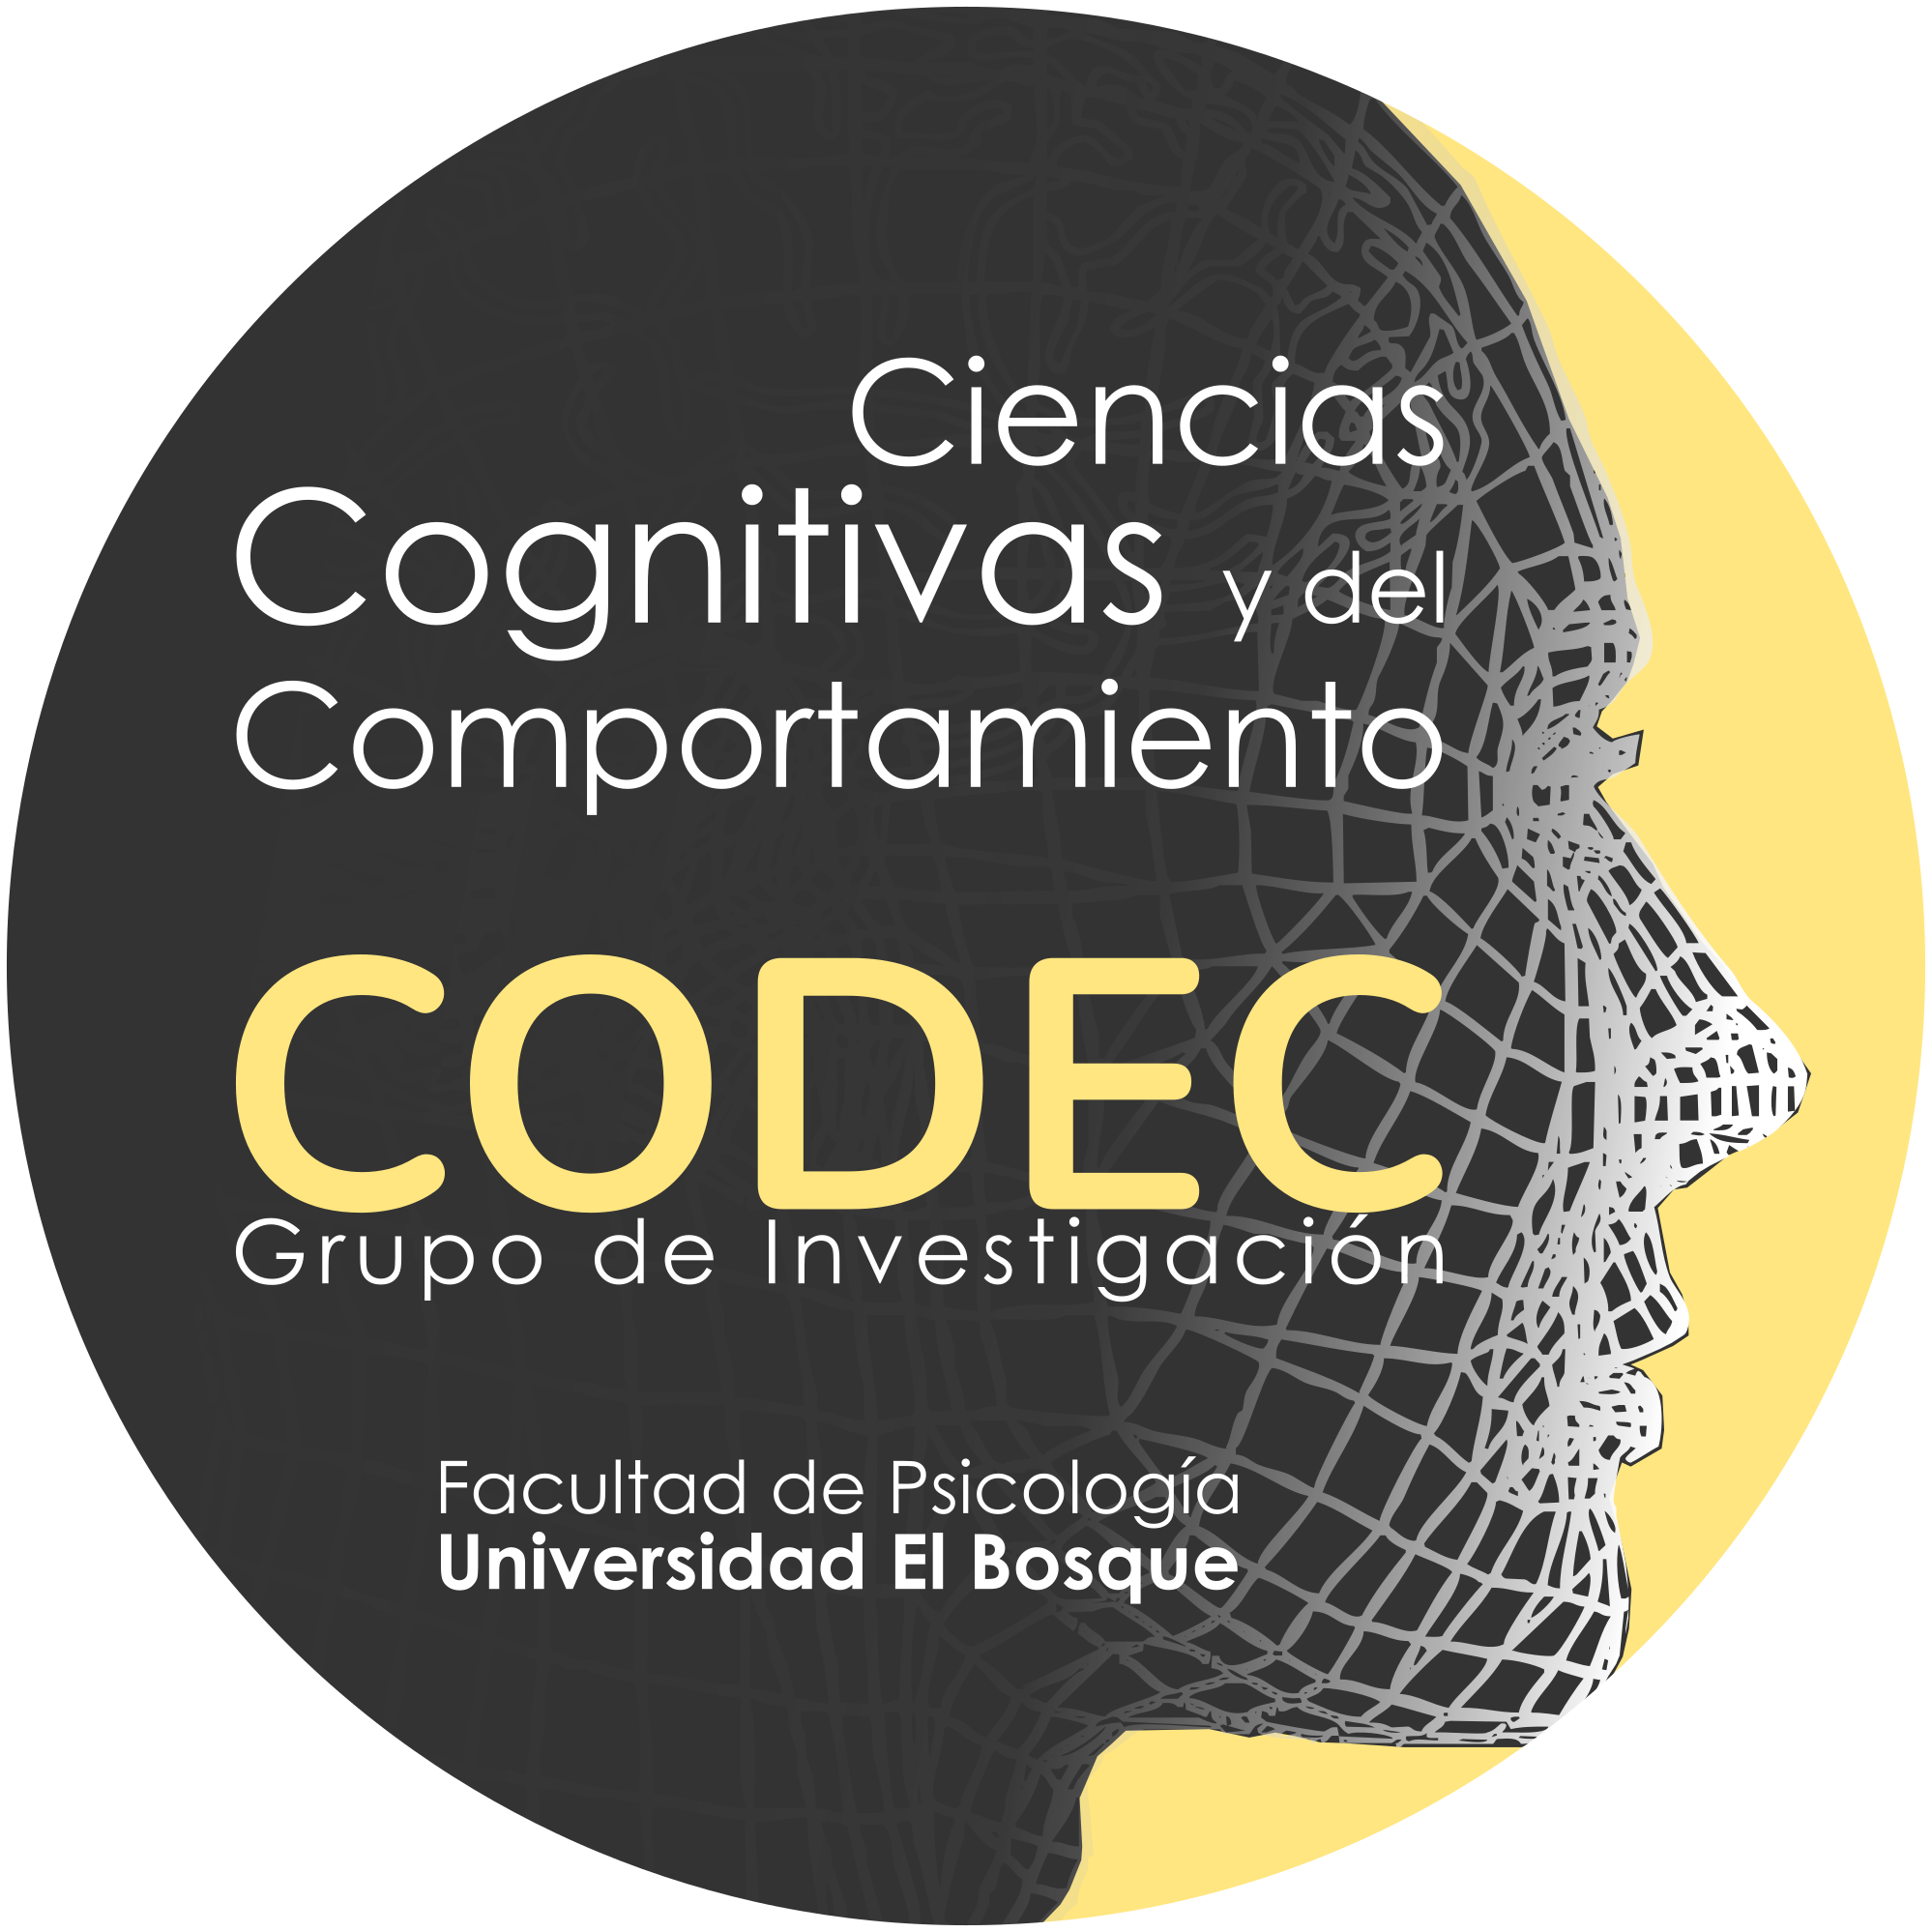
\includegraphics[width=2.3cm, height=2.3cm]{Logo_CODEC.png}}
\end{flushright}
\end{minipage}

\hypertarget{habilidades}{%
\section{Habilidades}\label{habilidades}}

\begin{cvskills}
  \cvskill
    {Programación}
    {\href{https://www.r-project.org/}{\textbf{R}} (Básico, análisis de datos y generación de gráficos)}

  \cvskill
    {Investigación cuantitativa}
    {Estudios observacionales-correlacionales, Modelos lineales generales simples y mixtos}
  
  \cvskill
    {Técnicas de registro}
    {Rastreo Ocular (principalmente), otras básicas HRV, EEG}

  \cvskill
    {Software}
    {RStudio, Tobii Pro Lab, Qualtrics, Psychomorph, WebmorphR, Mendeley y Zotero}

  \cvskill
    {Languages}
    {Español/Inglés}
\end{cvskills}

\hypertarget{investigaciuxf3n}{%
\section{Investigación}\label{investigaciuxf3n}}

\begin{cvskills}
  \cvskill
    {Áreas de investigación}
    {\textbf{Respuesta sexual humana • Preferencias sexuales típicas y atípicas • Pedohebefilia • Conductas \newline sexuales perjudiciales • Elección de pareja • Sesgos atencionales}}

  \cvskill
    {Principales métodos de investigación}
    {Diseños experimentales • Paradigmas de visualización libre y elección forzada de estímulos • Evaluación \newline subjetiva de estímulos visuales • Escalas psicométricos}
\end{cvskills}

\hypertarget{educaciuxf3n}{%
\section{Educación}\label{educaciuxf3n}}

\begin{cventries}
    \cventry{PhD - Neurociencias}{\href{https://www.uv.es/uvweb/universidad/es/universidad-valencia-1285845048380.html}{Universidad de Valencia}}{Valencia, España}{2018}{\begin{cvitems}
\item Proyecto de investigación: \href{https://producciocientifica.uv.es/documentos/5eb09d10299952764112462f}{\textbf{\textit{Preferencias sexuales típicas y atípicas según sexo y edad de los estímulosutilidad de la técnica de rastreo ocular}}}
\item Supervisores: \href{https://www.uv.es/labnsc/miembros\%20individualmente/miembrosaliciasalvador.html/}{Prof. Alicia Salvador}, y \href{https://jdleongomez.info/es/}{Prof. Juan David Leongómez}
\end{cvitems}}
    \cventry{Máster en Neurociencias Básicas y Aplicadas}{\href{https://www.uv.es/uvweb/universidad/es/universidad-valencia-1285845048380.html}{Universidad de Valencia}}{Valencia, España}{2012}{\begin{cvitems}
\item Producto de Investigación: \href{https://revistas.um.es/analesps/article/view/analesps.31.1.167241/169851}{\textbf{\textit{Efectos del entrenamiento asistido con neurofeedbacksobre el EEG, los procesos de fun-ción ejecutiva y el estado de ánimo en una muestra de población normal}}}
\item Supervisora: \href{https://www.researchgate.net/profile/Marien-Gadea}{Prof. Marien Gadea}
\end{cvitems}}
    \cventry{Psicología}{\href{https://www.ucatolica.edu.co/portal/Pregrado/psicologia/}{Universidad Cátolica de Colombia}}{Bogotá, Colombia}{2007}{\begin{cvitems}
\item Producto de investigación: \href{http://www.scielo.org.co/scielo.php?pid=S1794-99982009000200010&script=sci_arttext}{\textbf{\textit{Diseño del cuestionario de creencias referidas al consumo de alcohol para jóvenes universitarios}}}
\end{cvitems}}
\end{cventries}

\hypertarget{educaciuxf3n-complementaria-relevante}{%
\section{Educación complementaria
relevante}\label{educaciuxf3n-complementaria-relevante}}

\begin{cventries}
    \cventry{Diplomado en Diseño y Uso Pedagógico de Ambientes Virtuales de Aprendizaje Mediados por las TIC y las TAC}{Universidad El Bosque}{Bogotá, Colombia}{2020}{}\vspace{-4.0mm}
    \cventry{Diplomado en Docencia Universitaria}{Politécnico Superior de Colombia}{Bogotá, Colombia}{2019}{}\vspace{-4.0mm}
\end{cventries}

\hypertarget{experiencia-acaduxe9mica}{%
\section{Experiencia Académica}\label{experiencia-acaduxe9mica}}

\begin{cventries}
    \cventry{Profesora Asociada}{\href{https://www.unbosque.edu.co/}{Universidad El Bosque}}{Bogotá, Colombia}{2020-2024}{\begin{cvitems}
\item Trabajo de grado III (2020-2024)
\item Seminario de Profundización II (Maestría en Psicología) (2020)
\end{cvitems}}
    \cventry{Profesora Asistente}{\href{https://www.unbosque.edu.co/}{Universidad El Bosque}}{Bogotá, Colombia}{2015-2019}{\begin{cvitems}
\item Seminario de Profundización II (Maestría en Psicología) (2019)
\item Laboratorio de Neurociencias y comportamiento (2015 - 2019)
\item Laboratorio de Motivación y Emoción (2015-2019)
\item Laboratorio de Procesos Cognoscitivos (2015 - 2018)
\end{cvitems}}
    \cventry{Profesora catedrática}{\href{https://www.usbbog.edu.co/}{Universidad de San Buenaventura de Bogotá}}{Bogotá, Colombia}{2015}{\begin{cvitems}
\item Taller de profundización (Maestría en Neuropsicología)  (2019 - 2020)
\end{cvitems}}
    \cventry{Profesora tiempo completo}{\href{https://www.usbmed.edu.co/}{Universidad de San Buenaventura de Medellín - Sede Ibagué}}{Ibagué, Colombia}{2013-2014}{\begin{cvitems}
\item Bases de Neurociencias (2013 - 2014)
\item Neuropsicología I (2013 - 2014)
\item Neuropsicología II  (2013 - 2014)
\item Seminario de introducción a la práctica  (2013 - 2014)
\item Trabajo de grado  (2013 - 2014)
\end{cvitems}}
    \cventry{Profesora catedrática}{\href{https://www.uan.edu.co/es/}{Universidad Antonio Nariño}}{Bogotá, Colombia}{2013-2014}{\begin{cvitems}
\item Procesos Psicológicos Básicos II- Laboratorio (2014)
\item Motivación y Emoción (2014)
\item Aprendizaje y Memoria (2014)
\item Neurociencias III (2014)
\item Teorías de la personalidad (2013)
\item Seminario de investigación IV (2013)
\item Seminario Optativo IV- Sexualidad, género y cultura (2013)
\item Trabajo de grado (2013)
\end{cvitems}}
    \cventry{Profesora catedrática}{\href{https://www.ucatolica.edu.co/}{Universidad Cátolica de Colombia}}{Bogotá, Colombia}{2009}{\begin{cvitems}
\item Laboratorio de Neuroanatomia funcional (2009)
\item Laboratorio de Neuropsicología (2009)
\end{cvitems}}
\end{cventries}

\hypertarget{experiencia-en-investigaciuxf3n}{%
\section{Experiencia en
Investigación}\label{experiencia-en-investigaciuxf3n}}

\begin{cventries}
    \cventry{Profesor Asociado}{\href{https://www.unbosque.edu.co/}{Universidad El Bosque}}{Bogotá, Colombia}{Ene. 2020 - Actualmente}{\begin{cvitems}
\item Investigadora en \href{https://grupo-codec.netlify.app/people/}{Laboratorio de Psicología Experimental}
\item Directora del Semillero \href{https://grupo-codec.netlify.app/sexcog/}{Semillero de Investigación SexCog}
\item Supervisora de proyectos de investigación de pregrado y postgrado asociados con psicología
\end{cvitems}}
    \cventry{Profesora visitante}{\href{https://www.cuc.edu.co/}{Universidad de la Costa}}{Barranquilla, Colombia}{Dic. 2023 - Actualmente}{\begin{cvitems}
\item II Estancia postdoctoral financiada por Minciencias
\end{cvitems}}
    \cventry{Profesor Colaborador}{\href{https://www.universidadviu.com/co/maestria-universitaria-en-neuropsicologia-clinica}{Univiersidad Internacional de Valencia}}{Valencia, España}{Oct. 2023 - Actualmente}{\begin{cvitems}
\item Supervisión de trabajos de fin de máster relacionados con la neuropsicología clínica
\end{cvitems}}
    \cventry{Profesora visitante}{\href{https://www.cuc.edu.co/}{Universidad de la Costa}}{Valencia, España}{Ene. 2021 - Ene. 2023}{\begin{cvitems}
\item I Estancia postdoctoral financiada por Minciencias
\end{cvitems}}
    \cventry{Profesor Asistente}{\href{https://www.unbosque.edu.co/}{Universidad El Bosque}}{Bogotá, Colombia}{Ene.  2015 - Dic. 2019}{\begin{cvitems}
\item Investigadora en \href{https://grupo-codec.netlify.app/people/}{Laboratorio de Psicología Experimental}
\end{cvitems}}
    \cventry{Docente investigadora}{\href{https://www.usbmed.edu.co/}{Universidad de Sanbuenaventura de Medellín}}{Medellín, Colombia}{Ene. 2013 - Jun. 2015}{\begin{cvitems}
\item Investigadora en el Grupo de Investigación Psicología \& Neurociencias (2014 - 2015)
\item Supervisora de una proyectos de investigación de pregrado en Psicología Neuropsicología (2013 - 2014)
\item Líder de semillero Neurognosis (2013-2014)
\end{cvitems}}
\end{cventries}

\hypertarget{experiencia-profesional}{%
\section{Experiencia Profesional}\label{experiencia-profesional}}

\begin{cventries}
    \cventry{Asesora Científica externa}{\href{https://www.redpapaz.org/}{ONG RedPapaz}}{Bogotá, Colombia}{Sep. - Oct. 2022}{\begin{cvitems}
\item Consultoria en implementación de proyecto de prevención de abuso sexual contra menores \href{https://childhelplineinternational.org/te-guio/}{TeGuío Helpline}
\end{cvitems}}
    \cventry{Consultora científica internacional}{\href{https://www.suojellaanlapsia.fi/en}{Protect Children}}{Helsink, Finlandia}{Jul. - Ago. 2021}{\begin{cvitems}
\item Traducción y adaptación al español del \href{https://www.mielenterveystalo.fi/en/self-help/redirection-self-help-program-stop-using-csam}{Global ReDirection Program: Protecting Children Through Prevention}
\end{cvitems}}
    \cventry{Profesional Validador}{\href{https://https://www.areandina.edu.co/}{Fundación del area Andina}}{Bogotá, Colombia}{Sep. 2020 - Ene.2021}{\begin{cvitems}
\item Validador experto de Instrumento de selección para la provisión de empleos vacantes propias de convocatorias territoriales 2019-II
\end{cvitems}}
    \cventry{Profesional en Neuropsicología}{\href{https://web.facebook.com/ACYSTERAPIAS/}{Centro de Atención Terapéutica ACYS, Colombia}}{Bogotá, Colombia}{Ago. 2013 - Ene. 2021}{\begin{cvitems}
\item Evaluación neuropsicológica en niños, niñas y adolescentes
\end{cvitems}}
    \cventry{Psicóloga especialista en Neuropsicología}{\href{https://neurolearningterapias.com/nosotros/}{Organización de Terapia Integral Pavlov, Colombia }}{Bogotá, Colombia}{Ago. 2008 - Sept. 2009}{\begin{cvitems}
\item Evaluación y entrenamiento en Neurofeedback
\end{cvitems}}
\end{cventries}

\hypertarget{subvenciones}{%
\section{Subvenciones}\label{subvenciones}}

\begin{cventries}
    \cventry{\href{https://minciencias.gov.co/convocatorias/construccion-paz-programa-y-proyectos-ctei-fortalecimiento-capacidades-para-la}{Estancia Postdoctoral - Convocatoria 935-2023  - Programa orquídeas. Mujeres en la ciencia: agentes para la paz: Agentes para la Paz 2023}}{\href{https://minciencias.gov.co/}{Minciencias}}{Barranquilla, Colombia}{Dic. 2023 - Ene. 2025}{\begin{cvitems}
\item Proyecto: Efecto de la disponibilidad de recursos sobre las preferencias de las mujeres por la masculinidad de los rostros en interacción con factores hormonales, cognitivos, y socio-contextuales como la escasez de recursos real y la exposición a violencias: un estudio experimental usando eye-tracking
\item COP\$356.040.884
\end{cvitems}}
    \cventry{IX \href{https://www.unbosque.edu.co/centro-informacion/convocatoria/xiv-convocatoria-interna-de-investigaciones}{Convocatoria Interna para la Financiación de Proyectos de Investigación}, 2024}{\href{https://www.unbosque.edu.co/}{Universidad El Bosque}}{Bogota, Colombia}{Ene. 2024 - Ene. 2026}{\begin{cvitems}
\item Proyecto: Efecto del control de los recursos real y simulado sobre las preferencias de mujeres andrófilas por la masculinidad en rostros de hombres: un estudio experimental usando rastreo ocular
\item Rol: Investigadora principal
\item COP\$90.000.000
\end{cvitems}}
    \cventry{\href{https://minciencias.gov.co/convocatorias/oportunidades-formacion/convocatoria-programa-estancias-postdoctorales-en-entidades}{Estancia Postdoctoral - Convocatoria Programa de Estancias Postdoctorales en entidades del SNCTeI 2019}}{\href{https://minciencias.gov.co/}{Minciencias}}{Barranquilla, Colombia}{Ene. 2021 - Ene. 2022}{\begin{cvitems}
\item Proyecto: Viabilidad de nuevas intervenciones para mejorar la implementación de programas de salud sexual y reproductiva en Colombia
\item COP\$192.000.000
\end{cvitems}}
    \cventry{\href{https://minciencias.gov.co/convocatorias/vocaciones-cientificas-ctei/convocatoria-para-el-fortalecimiento-proyectos-en}{Convocatoria para el fortalecimiento de proyectos en ejecución de CTeI en ciencias de la salud con talento joven e impacto regional 2020}}{\href{https://minciencias.gov.co/}{Minciencias}}{Bogota, Colombia}{Ene. 2021 - Ene. 2022}{\begin{cvitems}
\item Proyecto: Sesgos atencionales y su relación con la variabilidad de la frecuencia cardíaca como predictores del estado emocional de personas sin trastornos afectivos de la ciudad de Bogotá
\item Rol: Investigadora principal
\item COP\$76.000.000
\end{cvitems}}
    \cventry{IX \href{https://www.unbosque.edu.co/investigaciones/convocatorias-investigacion}{Convocatoria Interna para la Financiación de Proyectos de Investigación}, 2017}{\href{https://www.unbosque.edu.co/}{Universidad El Bosque}}{Bogota, Colombia}{Ene. 2018 - Dic. 2021}{\begin{cvitems}
\item Proyecto: Señales perceptibles de salud física y mental en rostros, voces y olores corporales, y su relación con niveles hormonales
\item Rol: Co-investigadora
\item COP\$136.586.537
\end{cvitems}}
    \cventry{VII \href{https://www.unbosque.edu.co/investigaciones/convocatorias-investigacion}{Convocatoria Interna para la Financiación de Proyectos de Investigación}, 2015}{\href{https://www.unbosque.edu.co/}{Universidad El Bosque}}{Bogota, Colombia}{Ene. 2016 - Dic. 2019}{\begin{cvitems}
\item Proyecto: Diferencias en el patrón de rastreo ocular hacia estímulos sexualmente preferidos en hombres condenados por delitos sexuales y población en general
\item Rol: Investigadora principal
\item COP\$80.000.000
\end{cvitems}}
    \cventry{Convocatoria Interna de Investigación Financiera de la Universidad de San Buenaventura, 2014}{\href{https://www.usbmed.edu.co/}{Universidad San Buenaventura de Medellín}}{Medellín, Colombia}{Jun.2014 - Jun.2015}{\begin{cvitems}
\item Proyecto: Factores mediadores de la Reserva Cognitiva y su relación con el perfil neuropsicológico del adulto mayor en proceso de envejecimiento normal
\item Rol: Investigadora principal
\item COP\$20.000.000
\end{cvitems}}
\end{cventries}

\hypertarget{becas-premios-y-honores}{%
\section{Becas, Premios y Honores}\label{becas-premios-y-honores}}

\begin{cventries}
    \cventry{X Convocatoria de Estímulos a la Excelencia}{\href{https://www.unbosque.edu.co/}{Universidad El Bosque}}{Bogotá, Colombia}{Dic. 2023}{\begin{cvitems}
\item COP\$10.000.000
\end{cvitems}}
    \cventry{VIII Convocatoria de Estímulos a la Excelencia}{\href{https://www.unbosque.edu.co/}{Universidad El Bosque}}{Bogotá, Colombia}{Dic. 2019}{\begin{cvitems}
\item COP\$5.000.000
\end{cvitems}}
    \cventry{VII Convocatoria de Estímulos a la Excelencia}{\href{https://www.unbosque.edu.co/}{Universidad El Bosque}}{Bogotá, Colombia}{Dic. 2018}{\begin{cvitems}
\item COP\$2.500.000
\end{cvitems}}
    \cventry{Mención Cum Laude}{\href{https://www.uv.es/}{Universidad de Valencia}}{Valencia, España}{Sep. 2018}{\begin{cvitems}
\item Tesis doctoral en Neurociencias
\end{cvitems}}
    \cventry{Beca Luisa Cardona}{\href{https://https://www.uv.es/uvcooperacion/es/becas-ayudas/ayudas-estudiantes-paises-cooperacion/becas-luisa-cardona.html/}{Universidad de Valencia}}{Valencia, España}{Nov.2011 - Nov.2012}{\begin{cvitems}
\item Exención de tasas del Máster Oficial
\end{cvitems}}
    \cventry{Grado de Honor}{\href{https://www.ucatolica.edu.co/}{Universidad Cátolica de Colombia}}{Bogotá, Colombia}{Sep. 2007}{\begin{cvitems}
\item Mejor desempeño entre estudiantes de pregrado de Psicología
\end{cvitems}}
    \cventry{Mención de excelencia Facultad de Psicología}{\href{https://https://www.ucatolica.edu.co/portal/Facultades/facultad-de-psicologia/}{Universidad Cátolica de Colombia}}{Bogotá, Colombia}{Mar.2007}{\begin{cvitems}
\item Mención por obtener el puntaje más alto entre los estudiantes de psicología de la facultad y 3er lugar a nivel nacional en el Examen de Calidad de la Educación Superior en Colombia (ECAES) versión 2006
\end{cvitems}}
\end{cventries}

\hypertarget{publicaciones}{%
\section{Publicaciones}\label{publicaciones}}

\begin{tcolorbox}[enhanced,
        on line, 
        boxsep=4pt, left=0pt,right=0pt,top=0pt,bottom=0pt,
        colframe=white,colback=violet,
        hyperurl={https://scholar.google.com/citations?user=XgNEpfgAAAAJ}]
  
\color{white}
  \begin{minipage}[c]{0.245\linewidth}
    \begin{center} 
      \begin{huge} 7 \end{huge}
     \begin{small} Índice \textit{h} \end{small} 
    \end{center} 
  \end{minipage} 
  \begin{minipage}[c]{0.245\linewidth}
    \begin{center} 
      \begin{huge} 19 \end{huge}
      \begin{small} Índice \textit{g} \end{small} 
    \end{center}
  \end{minipage} 
  \begin{minipage}[c]{0.245\linewidth}
    \begin{center} 
      \begin{huge} 7 \end{huge}
      \begin{small} Índice i10 \end{small} 
    \end{center}
  \end{minipage} 
  \begin{minipage}[c]{0.245\linewidth}
    \begin{center}  
      \begin{huge} 20 \end{huge}
      \begin{small} Publicaciones \end{small} 
    \end{center}
  \end{minipage} 
  
  \begin{center} \noindent\line(1,0){150} Citas \noindent\line(1,0){150} \end{center}
  
  \begin{minipage}[c]{0.325\linewidth}  
    \begin{center} 
      \begin{small} Total \end{small} 
      \begin{LARGE} 386 \end{LARGE} 
    \end{center}
  \end{minipage} 
  \begin{minipage}[c]{0.325\linewidth}
    \begin{center} 
      \begin{small} Media \end{small} 
      \begin{LARGE} 19.3 \end{LARGE}
    \end{center}
  \end{minipage} 
  \begin{minipage}[c]{0.325\linewidth}
    \begin{center}  
      \begin{small} Mediana \end{small} 
      \begin{LARGE} 4.5 \end{LARGE}
   \end{center}
  \end{minipage} 
\end{tcolorbox}

\hypertarget{section}{%
\subsection{\texorpdfstring{\textbf{Artículos Publicados}}{}}\label{section}}

\begingroup
\footnotesize
\setlength{\parindent}{-0.5in}
\setlength{\leftskip}{0.5in}

\textbf{Vásquez-Amézquita, M.}, Leongoméz, J. D., Salvador, A., \& Seto,
M. C. (2023). What can the eyes tell us about atypical sexual
preferences as a function of sex and age? Linking eye movements with
child-related chronophilias. \emph{Forensic Sciences Research,
8}(1)1--11. \url{https://doi.org/10.1093/fsr/owad009}

\textbf{Vásquez-Amézquita, M.}, Salvador, A., \& Leongómez, J. D.
(2021). Existen diferencias en la ratio 2D:4D entre delincuentes
sexuales y no sexuales, y hombres no delincuentes? Un estudio en una
muestra colombiana. Interdisciplinaria. \emph{Revista de Psicología y
Ciencias Afines, 39}(1).
\url{https://doi.org/10.16888/interd.2022.39.1.8}

Leongómez, J. D., Sánchez, O. R., \textbf{Vásquez-Amézquita, M.}, \&
Roberts, S. C. (2021). Contextualising courtship: Exploring male body
odour effects on vocal modulation. \emph{Behavioural Processes, 193}
104531.
\url{https://doi.org/https://doi.org/10.1016/j.beproc.2021.104531}

Jones, B. C., DeBruine, L. M., Flake, J. K., Liuzza, M. T., Antfolk, J.,
Arinze, N. C., Ndukaihe, I. L. G., Bloxsom, N. G., Lewis, S. C., Foroni,
F., Willis, M. L., Cubillas, C. P., Vadillo, M. A., Turiegano, E.,
Gilead, M., Simchon, A., Saribay, S. A., Owsley, N. C., Jang, C. \ldots,
\textbf{Vásquez-Amézquita, M.}, \ldots, Coles, N. A. (2021). To which
world regions does the valence--dominance model of social perception
apply? Nature Human Behaviour, 5(1) 159-169.
\url{https://doi.org/10.1038/s41562-020-01007-2}

Leongómez, J. D., Sanchez, O. R., \textbf{Vásquez-Amézquita, M.},
Valderrama, E., Castellanos-Chacon, A., Morales-Sanchez, L., Nieto, J.,
\& Gonzalez-Santoyo, I. (2020). Self-reported Health is Related to Body
Height and Waist Circumference in Rural Indigenous and Urbanised
Latin-American Populations. \emph{Scientific Reports, 10}, 4391.
\url{https://doi.org/10.1101/562942}

\textbf{Vásquez-Amézquita, M.}, Leongómez, J. D., Seto, M. C., Bonilla,
F. M., Rodríguez-Padilla, A., \& Salvador, A. (2018). No relation
between digit ratio (2D:4D) and visual attention patterns to sexually
preferred and non-preferred stimuli. \emph{Personality and Individual
Differences, 120}, 151--158.
\url{https://doi.org/10.1016/j.paid.2017.08.022}

\textbf{Vásquez-Amézquita, M.}, Leongómez, J. D., Seto, M. C., Bonilla,
M., Rodríguez-Padilla, A., \& Salvador, A. (2019). Visual Attention
Patterns Differ in Gynephilic and Androphilic Men and Women Depending on
Age and Gender of Targets. \emph{The Journal of Sex Research, 56}(1),
85--101. \url{https://doi.org/10.1080/00224499.2017.1372353}

\textbf{Vásquez-Amézquita, M.}, Leongómez, J. D., Seto, M. C., \&
Salvador, A. (2019). Differences in Visual Attention Patterns to
Sexually Mature and Immature Stimuli Between Heterosexual Sexual
Offenders, Nonsexual Offenders, and Nonoffending Men. \emph{The Journal
of Sex Research, 56} (2), 213--228.
\url{https://doi.org/10.1080/00224499.2018.1511965}

\textbf{Vásquez-Amézquita, M.} (2016). Factores predictores de la
reserva cognitiva en un grupo de adultos mayores. \emph{Revista Chilena
de Neuropsicología, 11}(1), 5--11.
\url{https://doi.org/10.5839/rcnp.2016.11.01.02}

\textbf{Vásquez-Amézquita, M.}, Gadea, M., Garijo, E., Aliño, M., \&
Salvador, A. (2015). Effects of assisted training with neurofeedback on
EEG measures, executive function and mood in a healthy sample.
{[}Efectos del entrenam. asistido con neurofeedback sobre el EEG, los
procesos de función ejecutiva y el afecto en una muestra de pobl.
normal{]}. \emph{Anales de Psicología, 31}(1), 317-323.
\url{https://doi.org/10.6018/analesps.31.1.167241}

\textbf{Vásquez-Amézquita, M.}, Rodriguez, A., Villarreal, J. S., \&
Campos, A. (2014). Relación entre la Reserva Cognitiva y el
Enriquecimiento Ambiental: Una revisión del Aporte de las Neurociencias
a la comprensión del Envejecimiento Saludable. \emph{Panamerican Journal
of Neuropsychology, 8}(2), 171--201.
\url{https://doi.org/10.7714/cnps/8.2.203}

\endgroup

\hypertarget{section-1}{%
\subsection{\texorpdfstring{\textbf{Artículos en Revisión}}{}}\label{section-1}}

\begingroup
\footnotesize
\setlength{\parindent}{-0.5in}
\setlength{\leftskip}{0.5in}

\textbf{Vásquez-Amézquita, M.}, Leongómez, J.D., Martínez-González, M.
B., \& Chivers, M. L. (2023). \emph{Trait Sexual Desire-Linked
Subjective Sexual Arousal to Erotic and Non-Erotic Stimuli: Gender,
Relationship Status, and Gender-Specificity}. {[}Manuscript submitted
for publication{]}.

Roa, E. Torres, J.S., Leongómez, J.D., Martínez-González, M. B., \&
\textbf{Vásquez-Amézquita, M.} (2024). \emph{Influencia de la frecuencia
del uso de pornografía en la excitación sexual subjetiva, deseo sexual y
satisfacción sexual en hombres y mujeres cisgénero con pareja}.
{[}Manuscript submitted for publication{]}.

\endgroup

\hypertarget{presentaciones-en-conferencias-puxf3sters-y-talleress}{%
\section{Presentaciones en Conferencias, Pósters y
Talleress}\label{presentaciones-en-conferencias-puxf3sters-y-talleress}}

\begingroup
\footnotesize
\setlength{\parindent}{-0.5in}
\setlength{\leftskip}{0.5in}

\textbf{Vásquez-Amézquita, M.} (2024, Abril). \emph{Preferencias
sexuales humanas: Métodos experimentales y Rastreo ocular}. Presentación
invitada al Webinar organizado por Maestría en Sexualidad y Relaciones
Contemporáneas (Universidad de la Costa), Barranquilla, Colombia.

\textbf{Vásquez-Amézquita, M.} (2023, Octubre). \emph{Descifrando la
pedofilia, una perspectiva neurocognitiva}. Presentación invitada al
Conversatorio Trata de personas, tráfico de NNA y pedofilia (Pontificial
Universidad Javeriana), Bogotá, Colombia.

\textbf{Vásquez-Amézquita, M.} (2022, Octubre). \emph{Deseo sexual rasgo
como predictor de la excitación sexual subjetiva hacia estímulos
sexuales eróticos de hombres y mujeres cisgénero}. Comunicación Oral en
el XX Congreso Latinoamericano de Sexología y Educación sexual
(Flasses), Valencia, España.

\textbf{Vásquez-Amézquita, M.} (2021, Junio). \emph{Tecnología
Eye-Tracking aplicada a las disfunciones y desviaciones sexuales, como
la pedofilia}. Conferencista invitada al Congreso Online de Tecnologías
Aplicadas a la Psicología (AEPSIS - Asociación Española de Psicología
Sanitaria), Valencia, España.

\textbf{Vásquez-Amézquita, M.} (2020, Octubre). \emph{Aportes del Eye
tracking en la identificación de preferencias sexuales desviadas como la
pedofilia}. Conferencista invitada al II Congreso Internacional De
Psicología Online (Conexiones Consultorías, Universidad El Bosque y
ASCOFAPSI), Bogotá, Colombia.

\textbf{Vásquez-Amézquita, M.} (2020, Septiembre 17). \emph{Utilidad del
Eye-Tracking en la Identificación de Preferencias Sexuales en Población
General y Agresores Sexuales de Niños}. Conferencista invitada al IV
Congreso Nacional de Psicología Jurídica (Universidad Católica de
Colombia), Bogotá, Colombia.

\textbf{Vásquez-Amézquita, M.} (2020, Septiembre 4). \emph{¿Qué dice la
mirada acerca de comportamientos sexuales desviados como la pedofilia y
el abuso sexual infantil? Hallazgos de un estudio usando eye tracking}.
Conferencista invitada al 3er Simposio de Neurociencia, Cognición y
Sociedad (Pontificial Universidad Javeriana), Bogotá, Colombia.

\textbf{Vásquez-Amézquita, M.} (2020, Marzo). \emph{Contribuciones de la
neurociencia cognitiva en la identificación de preferencias sexuales
atípicas desviadas como la pedofilia}. Conferencista invitada a Sesión
plenaria en el CSCN -- Center for Social and Cognitive Neuroscience
(Universidad Adolfo Ibáñez), Santiago de Chile y Viña del Mar.

\textbf{Vásquez-Amézquita, M.} (2019, Octubre). \emph{Factores del
neurodesarrollo que contribuyen al desarrollo de la pedofilia}.
Conferencista invitada a I Simposio de Neuropsicología Infantil y
Neurociencias Aplicadas (Coorporación Delphy Colombia), Ibagué,
Colombia.

\textbf{Vásquez-Amézquita, M.} (2018, Septiembre). \emph{Patrón de
atención visual sobre los estímulos infantiles en abusadores sexuales de
niños en comparación con otros delincuentes y la comunidad en general:
un estudio de seguimiento ocular}. Conferencista invitada a 4º Congresso
Ordem dos Psicólogos Portugueses (Ordem Dos Psicólogos Portugueses),
Braga, Portugal.

\endgroup

\hypertarget{organizaciuxf3n-de-eventos-cientuxedficos}{%
\section{Organización de Eventos
Científicos}\label{organizaciuxf3n-de-eventos-cientuxedficos}}

\begin{cventries}
    \cventry{Organizadora y moderadora}{Conversatorio erotismo en pantalla: entre la ciencia y la subjetividad}{Universidad El Bosque - Fractales}{Mar. 15, 2024}{\begin{cvitems}
\item \href{https://www.youtube.com/watch?v=MRyZLaA96wo}{Fractales}
\end{cvitems}}
    \cventry{Presidente del Comité Organizador}{CIVN2020 - Congreso Internacional de Neurociencias: Cerebro y Comportamiento en Tiempos de COVID-19}{Universidad El Bosque y Universidad de los Andes}{Nov. 25 ‑ 28, 2020}{\begin{cvitems}
\item \href{http://doi.org/10.17605/OSF.IO/5BWNX}{Memorias}
\end{cvitems}}
\end{cventries}

\hypertarget{supervisiuxf3n-de-investigaciuxf3n}{%
\section{Supervisión de
Investigación}\label{supervisiuxf3n-de-investigaciuxf3n}}

\hypertarget{section-2}{%
\subsection{\texorpdfstring{\textbf{Posgrado}}{}}\label{section-2}}

La Facultad de Psicología de la Universidad El Bosque no ofrece títulos
de investigación, y todos los cursos de nivel de maestrías son
profesionales. Debido a esto, las oportunidades de supervisar a
estudiantes de posgrado son limitadas, y la mayor parte de mi
supervisión de posgrado ha sido externa.

\begin{cventries}
    \cventry{Máster en Neuropsicología Clínica}{Sara Silva Gómez}{\href{https://www.universidadviu.com/co/}{Universidad Internacional de Valencia}, España}{2022-2023}{\begin{cvitems}
\item Trabajo de grado: \textit{\href{https://repositorio.unbosque.edu.co/items/7d3fae16-e576-4380-99d0-1718b930a6bd}{Diseño de evaluación y rehabilitación neuropsicológica en pacientes con trastorno depresivo mayor tratados con terapia electroconvulsiva} [Evaluation design and neuropsychological rehabilitation in patients with major depressive disorder treated with electroconvulsive therapy]}
\end{cvitems}}
    \cventry{Máster en Neuropsicología Clínica}{Daniela Bermudez Calle}{\href{https://www.universidadviu.com/co/}{Universidad Internacional de Valencia}, España}{2022-2023}{\begin{cvitems}
\item Trabajo de grado: \textit{\href{https://repositorio.unbosque.edu.co/items/7d3fae16-e576-4380-99d0-1718b930a6bd}{Enfermedad de Huntington: una propuesta de intervención neuropsicológica en etapa inicial} [Huntington's disease: a proposal for early stage neuropsychological intervention]}
\end{cvitems}}
    \cventry{Máster en Neuropsicología Clínica}{Soraya López Aranda}{\href{https://www.universidadviu.com/co/}{Universidad Internacional de Valencia}, España}{2022-2023}{\begin{cvitems}
\item Trabajo de grado: \textit{\href{https://repositorio.unbosque.edu.co/items/7d3fae16-e576-4380-99d0-1718b930a6bd}{Plan de Evaluación e Intervención Neuropsicológica dirigido a adultos mayores institucionalizados en comparación con adultos mayores que asisten a centros de día} [Neuropsychological Assessment and Intervention Plan for institutionalized older adults compared to older adults attending day care centers]}
\end{cvitems}}
    \cventry{Máster en Neuropsicología Clínica}{Maite García Gil}{\href{https://www.universidadviu.com/co/}{Universidad Internacional de Valencia}, España}{2022-2023}{\begin{cvitems}
\item Trabajo de grado: \textit{\href{https://repositorio.unbosque.edu.co/items/7d3fae16-e576-4380-99d0-1718b930a6bd}{Diseño de intervención a través de estimulación cognitiva para la prevención del DCP en personas con discapacidad intelectual} [Design of intervention through cognitive stimulation for the prevention of CPD in people with intellectual disabilities]}
\end{cvitems}}
    \cventry{Máster en Neuropsicología Clínica}{Myrian García Martínez}{\href{https://www.universidadviu.com/co/}{Universidad Internacional de Valencia}, España}{2022-2023}{\begin{cvitems}
\item Trabajo de grado: \textit{\href{https://repositorio.unbosque.edu.co/items/7d3fae16-e576-4380-99d0-1718b930a6bd}{Plan de intervención integrando plataformas digitales y realidad virtual para la rehabilitación de la Enfermedad de Alzheimer en etapa moderada} [Intervention plan integrating digital platforms and virtual reality for the rehabilitation of moderate stage Alzheimer's disease]}
\end{cvitems}}
    \cventry{Maestría en Psicología}{Yenny Johanna Baron Londoño}{\href{https://www.unbosque.edu.co/}{Universidad El Bosque}, Colombia}{2019 - 2020}{\begin{cvitems}
\item Trabajo de grado: \textit{\href{https://repositorio.unbosque.edu.co/items/7d3fae16-e576-4380-99d0-1718b930a6bd}{Efecto De Los Niveles De Ansiedad Sobre Los Sesgos Atencionales Hacia Estímulos Emocionales Negativos En Adultos Jóvenes} [Effect of Anxiety Levels on Attentional Biases Toward Negative Emotional Stimuli in Young Adults]}
\end{cvitems}}
    \cventry{Maestría en Psicología}{Adrián Acosta Guerrero}{\href{https://www.unbosque.edu.co/}{Universidad El Bosque}, Colombia}{2019 - 2020}{\begin{cvitems}
\item Trabajo de grado \textbf{\textit{(Meritorio)}}: \textit{\href{http://hdl.handle.net/20.500.12495/4416}{La voz como predictor de sintomatología asociada a depresión y ansiedad} [Voice as a predictor of symptomatology associated with depression and anxiety]}
\end{cvitems}}
    \cventry{PhD en Psicología}{\href{https://www.neuroecologylab.com/doctorado-3/}{Juan Sebastián Lucero Carrasquilla}}{\href{https://www.unam.mx/}{Universidad Autonoma de México}, México}{2023 - En curso}{\begin{cvitems}
\item Tésis en curso: \textit{\href{https://cuved.unam.mx/divulgacion/index.php/CPMDP/XVICPPUNAM2022/paper/view/1623}{Correlatos Neurales en la Percepción de Rostros Humanos Sexualmente Dimórficos} [Neural Correlates in the Perception of Sexually Dimorphic Human Faces]}
\item Supervisión conjunta con Isaac González-Santoyo
\end{cvitems}}
\end{cventries}

\hypertarget{section-3}{%
\subsection{\texorpdfstring{\textbf{Pregrado}}{}}\label{section-3}}

Los estudiantes universitarios supervisados que figuran a continuación
proceden de distintas universidades y programas académicos. Esta lista
sólo incluye a los estudiantes de quienes fui supervisor principal u
obtuvieron mención a trabajo de grado meritorio. Adicionalmente,
actualmente estoy supervisando seis estudiantes como supervisor
principal, y he supervisado a más de 25 estudiantes como co-supervisor.

\begin{cventries}
    \cventry{Psicología}{Emily Valentina Roa Reatiga y Juan Sebastián Torres Herrera}{\href{https://www.unbosque.edu.co/}{Universidad El Bosque}, Colombia}{2023 - 2024}{\begin{cvitems}
\item \textbf{\textit{Trabajo de grado meritorio}}: 
\textit{Influencia de la frecuencia del uso de pornografía en la excitación, deseo y satisfacción sexual en hombres y mujeres con pareja}
\end{cvitems}}
    \cventry{Psicología}{Valentina Cepeda Monsalve}{\href{https://www.unbosque.edu.co/}{Universidad El Bosque}, Colombia}{2022 - 2023}{\begin{cvitems}
\item \textbf{\textit{Trabajo de grado meritorio}}: 
\textit{Pensamientos negativos hacia estímulos sexuales y su efecto sobre la atención a estímulos eróticos en hombres y mujeres cisgénero}
\end{cvitems}}
    \cventry{Psicología}{María Paula Díaz y Camila Galeano}{\href{https://www.unbosque.edu.co/}{Universidad El Bosque}, Colombia}{2021 - 2022}{\begin{cvitems}
\item Trabajo de grado: \textit{El rol de los pensamientos automáticos en la respuesta sexual humana – revisión teórica}
\end{cvitems}}
    \cventry{Psicología}{Laura Saenz Vanegas, Sofía Noriega Rey, y Daniela Hueso Fajardo}{\href{https://www.unbosque.edu.co/}{Universidad El Bosque}, Colombia}{2020 - 2021}{\begin{cvitems}
\item Trabajo de grado: \textit{El atractivo de lo erótico: diferencias en el patrón de atención visual sobre estímulos eróticos y no eróticos de hombres heterosexuales}
\end{cvitems}}
    \cventry{Psicología}{Clara Valentina Rendón Martínez}{\href{https://www.unbosque.edu.co/}{Universidad El Bosque}, Colombia}{2018 - 2019}{\begin{cvitems}
\item Trabajo de grado: \textit{Sesgos atencionales según la edad del estímulo hacia distractores sexuales durante una tarea cognitiva en universitarios }
\end{cvitems}}
    \cventry{Psicología}{Valeria Uribe y Daniela Arias}{\href{https://www.unbosque.edu.co/}{Universidad El Bosque}, Colombia}{2018 - 2019}{\begin{cvitems}
\item \textbf{\textit{Trabajo de grado meritorio}}: 
\textit{¿Predice la VFC los sesgos atencionales negativos a estímulos emocionales de personas sin trastornos afectivos?}
\end{cvitems}}
    \cventry{Psicología}{Cristina Andrade y Jhoana Andrea Ángel}{\href{https://www.unbosque.edu.co/}{Universidad El Bosque}, Colombia}{2018 - 2019}{\begin{cvitems}
\item Trabajo de grado: \textit{Efecto del contenido emocional de los estímulos sobre el patrón de atención visual temprano y tardío en personas sin trastornos afectivos: un estudio piloto con eye-tracking}
\end{cvitems}}
    \cventry{Psicología}{Angela Isabel Jiménez Machado}{\href{https://www.unbosque.edu.co/}{Universidad El Bosque}, Colombia}{2017 - 2019}{\begin{cvitems}
\item \textbf{\textit{Trabajo de grado meritorio}}: 
\textit{Diferencias en Proporción 2D:4D entre delincuentes sexuales, no sexuales y población general}
\end{cvitems}}
    \cventry{Psicología}{Gustavo Andrés Castellanos}{\href{https://www.unbosque.edu.co/}{Universidad El Bosque}, Colombia}{2017 - 2018}{\begin{cvitems}
\item \textbf{\textit{Trabajo de grado meritorio}}: 
\textit{ Diferencia en los patrones de atención visual en mujeres según la disponibilidad de recursos: Un estudio de eye-tracking}
\end{cvitems}}
    \cventry{Psicología}{Jorge Enrique Torres}{\href{https://www.unbosque.edu.co/}{Universidad El Bosque}, Colombia}{2017 - 2018}{\begin{cvitems}
\item \textbf{\textit{Trabajo de grado meritorio}}:
 \textit{Comparación del Efecto de Paradigmas Experimentales Con y Sin Distractores No Sexuales en la Identificación de Preferencias Sexuales Según la Edad de los Estímulos en Hombres Heterosexuales}
\end{cvitems}}
    \cventry{Psicología}{Ileana Andrea Parra}{\href{https://www.unbosque.edu.co/}{Universidad El Bosque}, Colombia}{2017 - 2018}{\begin{cvitems}
\item Trabajo de grado: \textit{Estudio de las preferencias sexuales según el índice de masa corporal femenino utilizando la técnica de rastreo ocular}
\end{cvitems}}
    \cventry{Psicología}{Michelle Jiménez Lafont}{\href{https://www.unbosque.edu.co/}{Universidad El Bosque}, Colombia}{2016 - 2017}{\begin{cvitems}
\item Trabajo de grado: \textit{Relación entre la proporción 2D:4D y la orientación sexual, agresión y fantasías sexuales en población universitaria?}
\end{cvitems}}
    \cventry{Psicología}{Laura Patricia Lozano Sapuy y Andrea Ángel Albarracín}{\href{https://www.usbmed.edu.co/}{Universidad San Buenaventura de Medellín}, Colombia}{2014 - 2015}{\begin{cvitems}
\item Trabajo de grado: \textit{Apego parental y su relación con el apego romántico y la dependencia afectiva en 119 universitarios de la ciudad de Ibagué Colombia}
\end{cvitems}}
    \cventry{Psicología}{Stefania García y Camila Remicio}{\href{https://www.usbmed.edu.co/}{Universidad San Buenaventura de Medellín}, Colombia}{2013 - 2014}{\begin{cvitems}
\item Trabajo de grado: \textit{Descripción de la respuesta afectiva a través de inducción emocional con imágenes y relación con la función ejecutiva en niños con inatención y conducta hiperactiva en etapa escolar}
\end{cvitems}}
    \cventry{Psicología}{Stywear Villamil}{\href{https://www.usbmed.edu.co/}{Universidad San Buenaventura de Medellín}, Colombia}{2013 - 2014}{\begin{cvitems}
\item Trabajo de grado: \textit{Relación entre el nivel de consumo de alcohol y el rendimiento en procesos de función ejecutiva en estudiantes universitarios entre los 18 y 25 años}
\end{cvitems}}
\end{cventries}



\end{document}
